\subsection{Diff-Pair Integrator (DPI) Synapse}

\begin{figure}
    \centering
    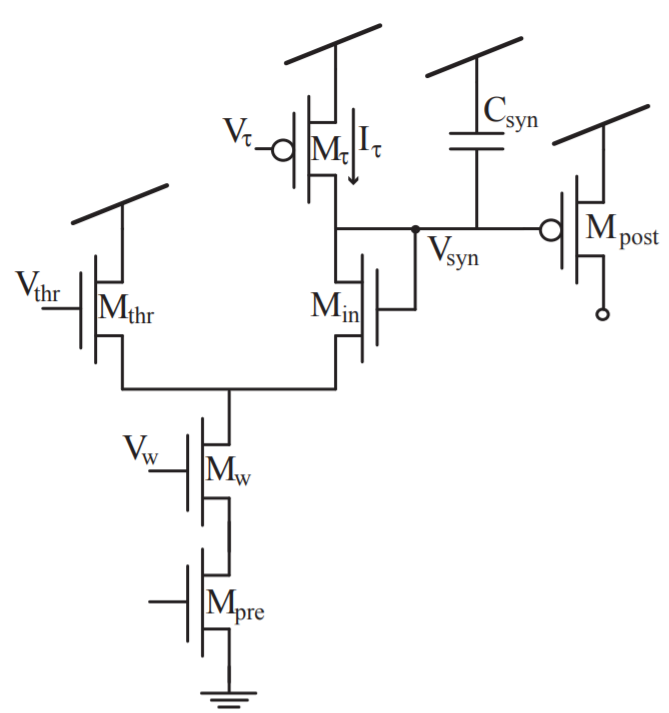
\includegraphics[width=.7\linewidth]{Figures/dpi_synpase.PNG}
    \caption{VLSI circuit of a diff-pair integrator (DPI) synapse.}
    \label{fig:dpi_synapse}
\end{figure}

\begin{figure}
    \centering
    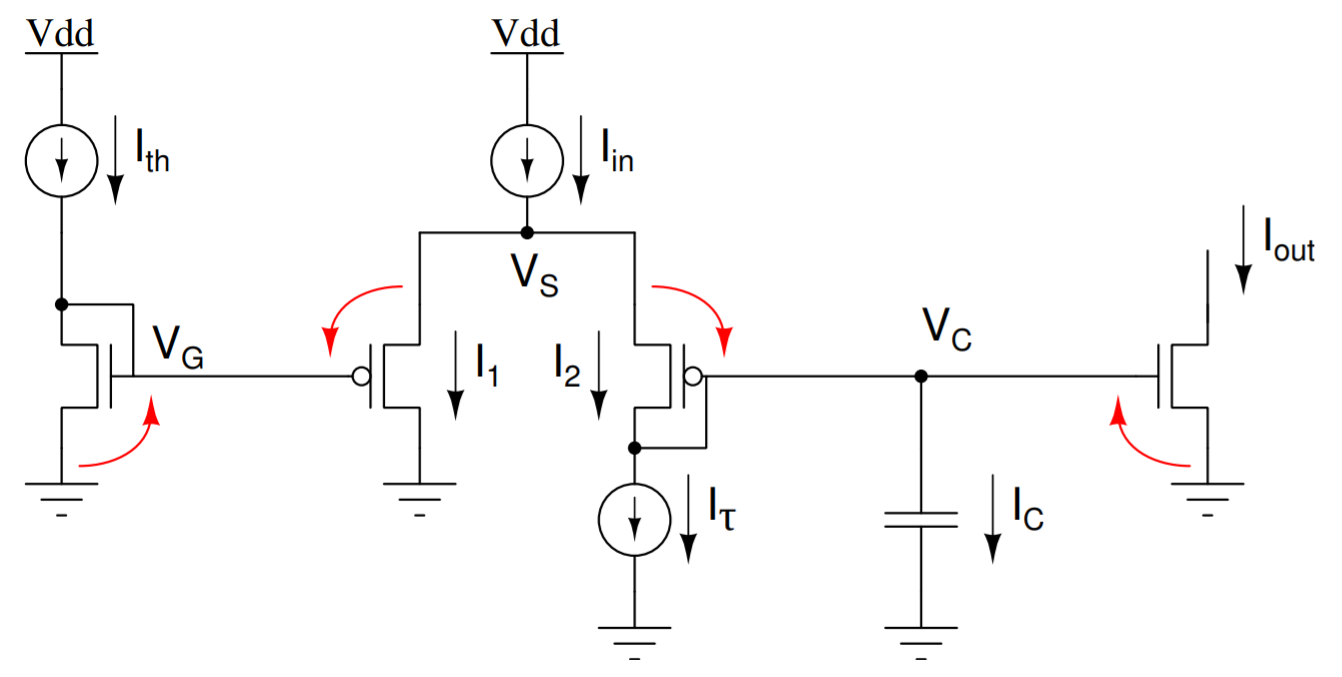
\includegraphics[width=\linewidth]{Figures/dpi_synapse_complementary.PNG}
    \caption{Complementary VLSI circuit of the DPI synapse.}
    \label{fig:dpi_synapse_complementary}
\end{figure}

The diff-pair integrator (DPI) synapse is visualized in figure \ref{fig:dpi_synapse}. It is named after its main component, a differential pair circuit. In order to understand its behaviour, we will analyze its complementary circuit shown in figure \ref{fig:dpi_synapse_complementary} instead. The circuit in figure  has the advantage that we can apply the translinear principle to it. The principle states that all gate-to-source voltages within a closed loop add up to zero. Note that the arrows always show from the source to the drain of the transistor. We get the following sum of voltages:

\begin{equation}
    (V_g - 0) - (V_g - V_s) + (V_c - V_s) - V_c = 0
\end{equation}

As we have seen in chapter \ref{sec:translinear_principle}, we can transform the above sum to a product of currents. Note that when we subtract the gate voltage of a pFET, we multiply the \textbf{positive} current of the corresponding transistor. We therefore get:

\begin{equation}
    I_{th} I_1 I_2^{-1} I_{out}^{-1} = 1 \implies I_{th} I_1 = I_2 I_{out}
\end{equation}

Because of Kirchhoff's current law, we know that: $I_{in} = I_1 + I_2$ and $I_2 = I_{\tau} + I_c$. We replace the currenst in above equation and get:

\begin{equation}
    I_{th} (I_{in} - I_{\tau} - I_c) = (I_{\tau} + I_c) I_{out}\label{eq:dpi_1}
\end{equation}

Now we would like to find an alternative equation for $I_c$ that is independent of the voltage.

\begin{equation}
    I_{out} = I_0 e^{\frac{\kappa V_c}{U_T}}
\end{equation}

\begin{equation}
    \frac{d}{dt} I_{out} = I_{out} \frac{\kappa}{U_T} \frac{d}{dt} V_c \implies\frac{d}{dt} V_c = \frac{d}{dt} I_{out} \frac{U_T}{\kappa I_{out}}
\end{equation}

\begin{equation}
    I_c = C \frac{d}{dt} V_c \implies I_c = C \frac{U_T}{\kappa I_{out}} \frac{d}{dt} I_{out}
\end{equation}

By inserting this equation into \eqref{eq:dpi_1} and rearranging, we get the following nonlinear differential equation for our output current:

\begin{equation}
    \tau (1 + \frac{I_{th}}{I_{out}}) \frac{d}{dt} I_{out} + I_{out} = \frac{I_{th} I_{in}}{I_{\tau}} - I_{th}\label{eq:dpi_2}
\end{equation}

where $\tau = \frac{C U_T}{\kappa I_{\tau}}$. So what happens now when we get a positive input current $I_{in}$? As soon as $I_{in}$ becomes larger than $I_{\tau}$, the capacitor is being charged. This leads to a linear increase of $V_c$, assuming a constant current input. Due to the exponential relationship between gate voltage and current, $I_{out}$ consequently starts to increase exponentially. As $I_{th}$ is a constant, the term $\frac{I_{th}}{I_{out}}$ in the above equation eventually becomes zero when we have an input current. Similarly, the term $I_{th}$ on the right hand side of the equation becomes negligible for $I_{in} \gg I_{\tau}$ as $\frac{I_{in}}{I_{\tau}} \gg 1$. We can therefore simplify \eqref{eq:dpi_2} to the following linear differential equation:

\begin{equation}
    \text{If $I_{in} \gg I_{\tau}$}: \tau \frac{d}{dt} I_{out} + I_{out} = \frac{I_{th}}{I_{\tau}} I_{in}
\end{equation}

Unlike the previously introduced circuits in section \ref{sec:exponentially_decaying_integrator} and \ref{sec:log_domain_pulse_integrator}, the behaviour of our synapse is now dependent on a variable current, $I_{th}$. This allows us to easily control our circuit's output.\\

There are two important things to note about the derived circuit. For simplicity, we previously assumed that $\kappa = 1$. However, in reality $\kappa$ is usually around $0.7$. In the DPI synapse, it turns out that all $\kappa$ values cancel each other out. We therefore only have to ensure that all $\kappa$ values are equal, in particular $\kappa_N = \kappa_P$ but we do not have to assume that $\kappa = 1$ anymore. Consequently, our derived equations very precisely model the circuit's actual behaviour. Another observation we make is that our calculations exploit the linear range of operation of the circuit's differential pair. We therefore have to ensure that $V_g$ and $V_s$ are within a similar range, i.e. that $|V_g - V_s|$ is small.\\

Let's have a look at our DPI synapse in figure \ref{fig:dpi_synapse} again. Based on the same derivations, its behaviour can be modelled by the same linear differential equation:

\begin{equation}
    \text{If $I_w \gg I_{\tau}$}: \tau \frac{d}{dt} I_{syn} + I_{syn} = \frac{I_{thr}}{I_{\tau}} I_{th}
\end{equation}

where $\tau = \frac{C U_T}{\kappa I_{\tau}}$. The only difference is that our input current $I_{in}$ is represented by the weighted current $I_w$. Our resulting circuit provides a biologically plausible and controllable model of a cortical synapse.

\subsubsection{Short-term Depression}\label{sec:short_term_depression}

\begin{figure}
    \centering
    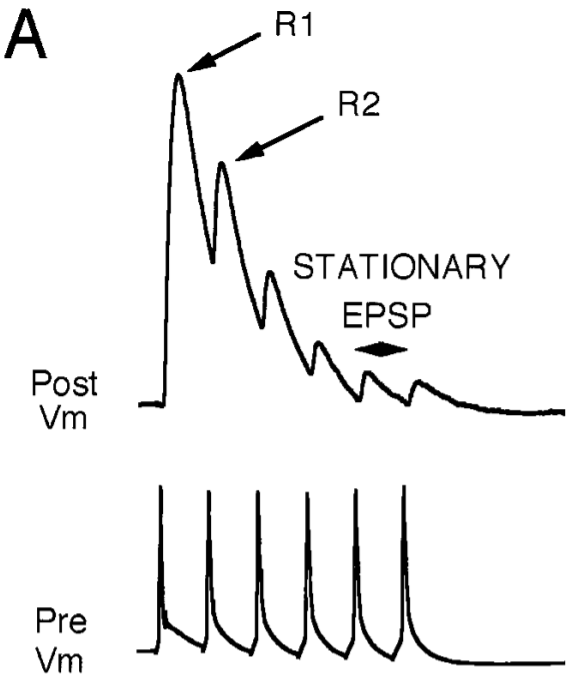
\includegraphics[width=.4\linewidth]{Figures/short_term_depression_data.PNG}
    \caption{Membrane voltage of a pre- and postsynaptic neuron that undergo short-term depression.}
    \label{fig:short_term_depression_data}
\end{figure}

In biological systems, the response of a synapse decreases when it receives input spikes at a high rate. This phenomenon is called short-term depression. It is visualized in figure \ref{fig:short_term_depression_data}. At the bottom of the figure, we see the firing pattern of the presynaptic neuron. As shown at the top of the figure, the synaptic information the postsynaptic neuron receives continuously decreases with every incoming spike.  By using two different transistors $M_{pre}$ and $M_w$ to separate our input pulse from its weight, we are actually able to implement this behaviour by replacing $V_w$ with an additional circuit. This circuit is shown in figure \ref{fig:short_term_depression_circuit}.\\

\begin{figure}
    \centering
    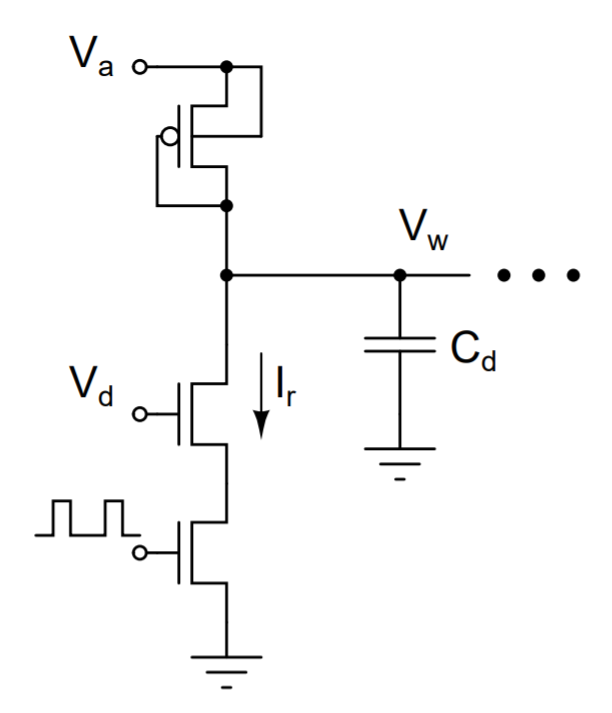
\includegraphics[width=.5\linewidth]{Figures/short_term_depression_circuit.PNG}
    \caption{VLSI circuit that implements short-term depression.}
    \label{fig:short_term_depression_circuit}
\end{figure}

The bottom transistor receives the same input pulse as our transistor $M_{pre}$ in the DPI synapse. Whenever we receive a pulse, i.e. an increase of the gate voltage, we generate a current $I_r$. This current flows out of the capacitor $C_d$, consequently discharging it and reducing the capacitor's voltage $V_w$. This is the voltage we use as the weighting gate voltage in our DPI synapse. The more pulses we receive, the more current flows out of the capacitor and the lower $V_w$ becomes. When we don't receive any input pulses, the diode $V_a$ eventually charges up the capacitor again and we retrieve our initial weighting voltage $V_w$.\\

\begin{figure}
\centering
\begin{subfigure}{.5\textwidth}
  \centering
  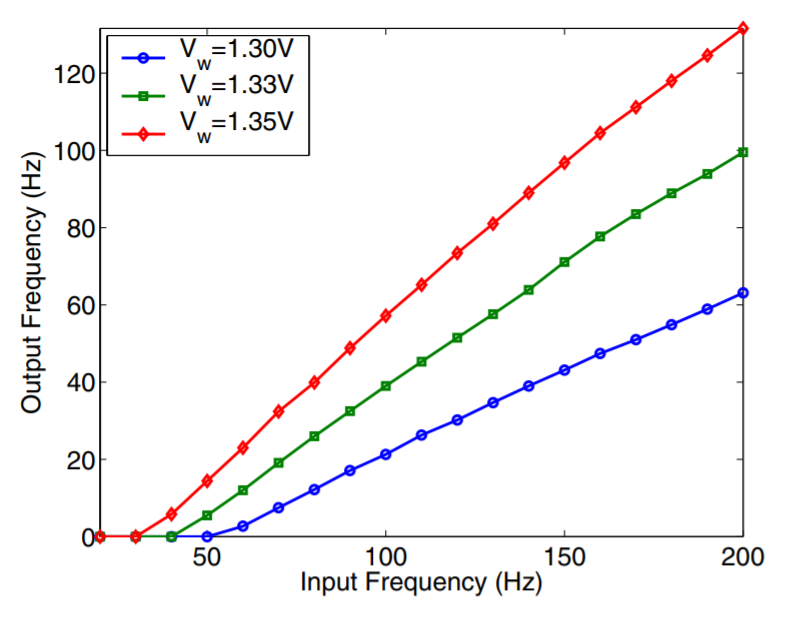
\includegraphics[width=\linewidth]{Figures/relu_dpi.PNG}
  \label{fig:relu_dpi}
\end{subfigure}%
\begin{subfigure}{.5\textwidth}
  \centering
  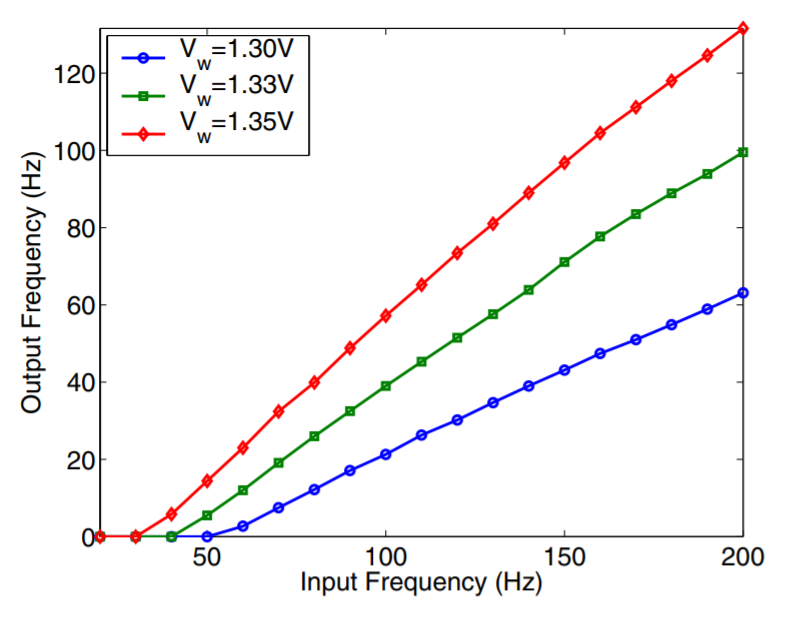
\includegraphics[width=\linewidth]{Figures/relu_dpi.PNG}
  \label{fig:relu}
\end{subfigure}
\caption{The response of the DPI synapse to a spike train (left) and the Rectified Linear Unit (ReLU) function (right).}
\end{figure}

There is one very interesting thing to note when comparing the frequency of our input pulses with the frequency of our output spikes. This relationship is shown in \ref{fig:relu_dpi}. First of all, the impact of our weight onto our output becomes clear. As expected, the higher our weight, the higher our output frequency. But more importantly - does the shape of the graph look familiar to you? Exactly, it is a ReLU function! For those unfamiliar with it, the ReLU (Rectified Linear Unit) function is an activation function that is very commonly used in neural networks. Its output is zero for any negative input or the positive input itself. Its shape is shown in figure \ref{fig:relu}. So why don't we simply use a ReLU function instead of our complex synapse circuit? When we are only interested in applying a ReLU activation onto our inputs, this is indeed the better way. The introduced synapse circuits, however, allow us to incorporate more complex dynamic behaviour that also occurs in biological synapses.